\documentclass[pdftex,12pt,a4paper]{article}

\usepackage{graphicx}  
\usepackage[margin=2.5cm]{geometry}
\usepackage{breakcites}
\usepackage{indentfirst}
\usepackage{pgfgantt}
\usepackage{pdflscape}
\usepackage{float}
\usepackage{epsfig}
\usepackage{epstopdf}
\usepackage[cmex10]{amsmath}
\usepackage{stfloats}
\usepackage{multirow}

\renewcommand{\refname}{REFERENCES}
\linespread{1.3}

\usepackage{mathtools}
%\newcommand{\HRule}{\rule{\linewidth}{0.5mm}}
\thispagestyle{empty}
\begin{document}
\begin{titlepage}
\begin{center}
\textbf{}\\
\textbf{\Large{ISTANBUL TECHNICAL UNIVERSITY}}\\
\vspace{0.5cm}
\textbf{\Large{COMPUTER ENGINEERING DEPARTMENT}}\\
\vspace{2cm}
\textbf{\Large{BLG 242E\\ DIGITAL CIRCUITS LABORATORY\\ EXPERIMENT REPORT}}\\
\vspace{2.8cm}
\begin{table}[ht]
\centering
\Large{
\begin{tabular}{lcl}
\textbf{EXPERIMENT NO}  & : & 8 \\
\textbf{EXPERIMENT DATE}  & : & 12.04.2019 \\
\textbf{LAB SESSION}  & : & FRIDAY - 14.00 \\
\textbf{GROUP NO}  & : & G13 \\
\end{tabular}}
\end{table}
\vspace{1cm}
\textbf{\Large{GROUP MEMBERS:}}\\
\begin{table}[ht]
\centering
\Large{
\begin{tabular}{rcl}
{
150180704  & : & C\.{I}HAT AKK\.{I}RAZ \\
150180707  & : & FAT\.{I}H ALTINPINAR \\
150180734  & : & S\.{I}NAN \c{S}AR \\
}
\end{tabular}}
\end{table}
\vspace{2.8cm}
\textbf{\Large{SPRING 2019}}

\end{center}

\end{titlepage}

 

\thispagestyle{empty}
\centering{\LARGE{ \textbf{ETHIC FORM}}}\\
\centering{\LARGE{\textbf{for}}}\\
\centering{\LARGE{\textbf{BLG242E Logic Circuits Laboratory}}}\\[0.2cm]
As a student of \\Istanbul Technical University Faculty of Computer and Informatics Engineering;
\begin{enumerate}
    \item I will not attempt to cheat in quizes and final exam,
    \item I will not use disallowed sources or tools (mobile phone, calculator etc.) during the exam,
    \item I will not write any information (formula, text, figure etc.) on the table, sheets or books that are allowed to be used during the exam,
    \item I will give reference when using printed or online published sources,
    \item I will not use the results in a source as they are, or by changing a part of them without giving a reference,
    \item I will not show unused sources as used, 
    \item I will not present someone else’s idea as my own idea, 
    \item I will not make someone do my homework, project or thesis for money or anything else,
    \item I will not take an exam or enter a lecture on behalf of others,
    \item I will not make excuses for not attending in exams or lessons by taking reports from someone I know (medical doctor parents or relatives),
    \item I will refrain from deliberately harming the public materials at our university,  
    \item I will comply with the safety rules in laboratory work,
    \item I will behave in accordance with the rules of respect for the lecturers and teaching assistants
\end{enumerate}
\vspace{-1em}
\centering{\LARGE{signed by}}\\
\vspace{-1em}
\begin{table}[ht]
\centering
\begin{tabular}{rcl}
150180704  & : & C\.{I}HAT AKK\.{I}RAZ \\
150180707  & : & FAT\.{I}H ALTINPINAR \\
150180734  & : & S\.{I}NAN \c{S}AR \\
\end{tabular}
\end{table}
\vspace{-1em}
 \begin{table}[ht]
 \begin{tabular}{lr}
%\textbf{Date:\hspace*{1.0cm}/\hspace*{1.0cm}/} &\qquad \qquad\qquad\qquad \qquad\qquad\qquad \qquad\qquad\qquad \qquad\qquad \textbf{SIGNED}\\
\end{tabular}
\end{table} % adds the ethic sign
\addcontentsline{toc}{section}{\numberline {}ETHICS}
 

\thispagestyle{empty}
\addtocontents{toc}{\contentsline {section}{\numberline {}FRONT COVER}{}}
\addtocontents{toc}{\contentsline {section}{\numberline {}CONTENTS}{}}
\setcounter{tocdepth}{4}
\tableofcontents
\clearpage

\setcounter{page}{1}

\section{INTRODUCTION}
\begin{flushleft}
\paragraph {}
In this experiment, several circuits are built in order to understand how counters function. Also an analysis is done for a given circuit as well.

In this experiment, several circuits are implemented in order to understand how sequencial circuits work, how they can be analyized nasil yaziliyo lan 

%  susu bosver jasldasd
\end{flushleft}

\section{REQUIREMENTS}
\begin{flushleft}
\underline{Tools Used}\cite{booklet}
\end{flushleft}

\begin{itemize}
    \item C.A.D.E.T
    \item 74000 series ICs
    \begin{itemize}
        \item 74xx04 - Hex Inverters
        \item 74xx08 - Quadruple 2-input Positive AND Gates
        \item 74xx32 - Quadruple 2-input Positive OR Gates
        \item 74xx161 - Synchronous 4-Bit Binary Counter
        \item 74xx174 - Hex D-Type Flip-Flops
    \end{itemize}
\end{itemize}

\begin{flushleft}
\subsection{PART 1}

\paragraph{}
In the first part of the experiment,  the circuit is implemented as shown in the figure below. X input connected to a logic switch and the clock is connected to a debounced pushbutton.  The output Y and flip-flop states are observed using LEDs on the logic monitor. 

\begin{figure}[h]
	\centering
	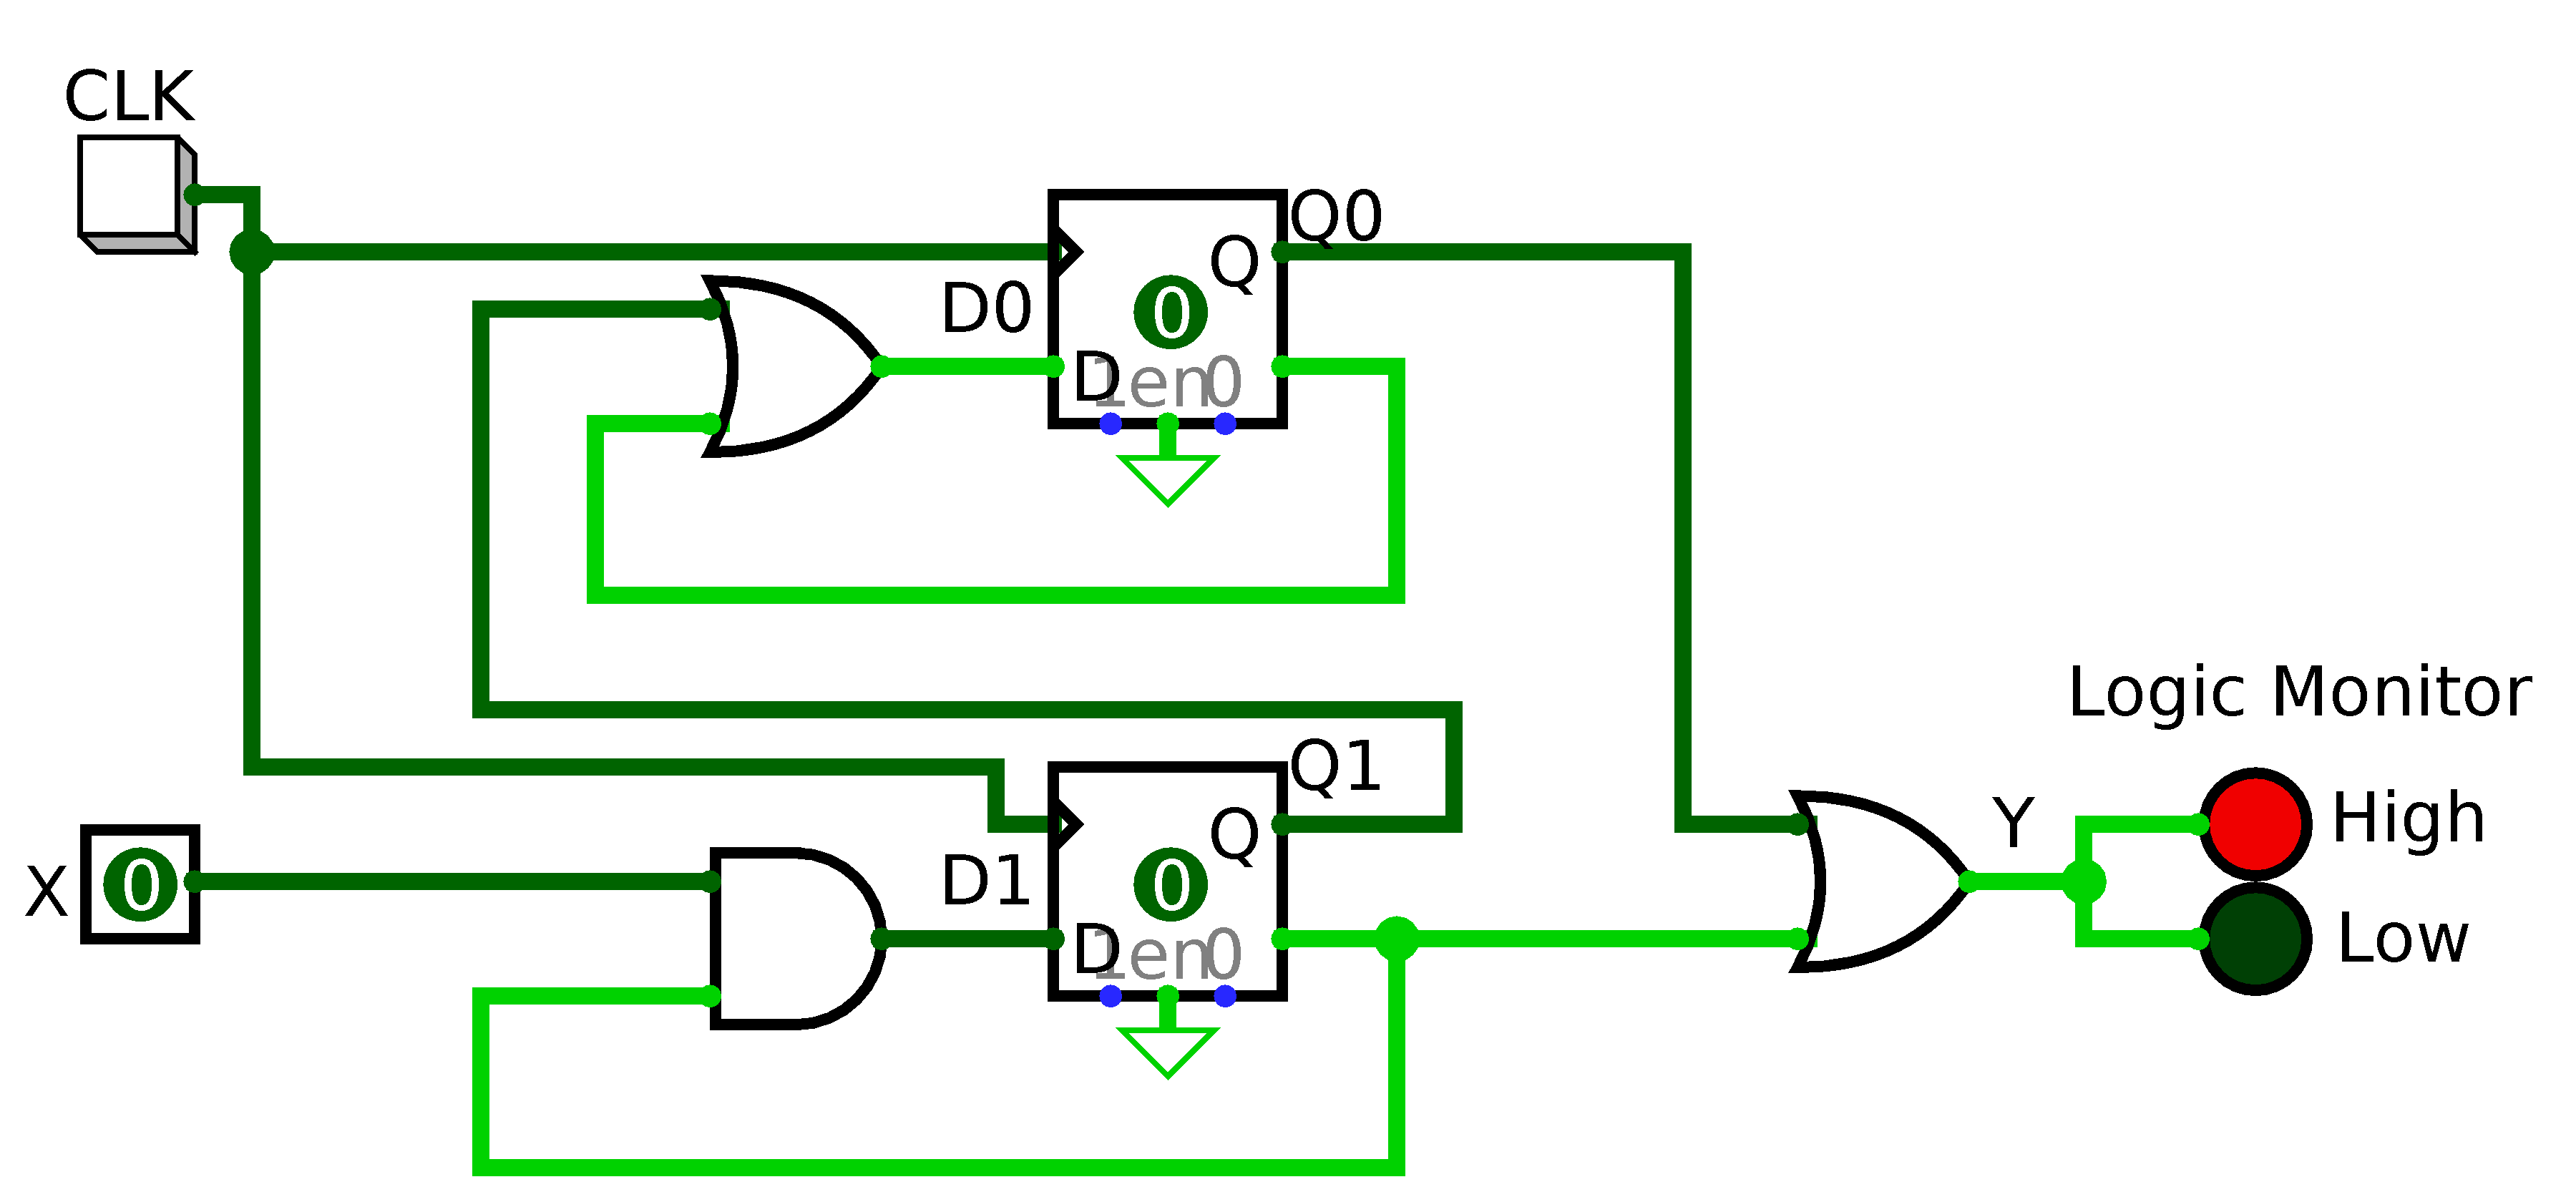
\includegraphics[width=0.7\textwidth]{part1.png}	
	\caption{Circuit that is implemented in Part 1}
	\label{circ:part1}
\end{figure}


% D_{0}
% D_{1}
% \bar{D_{0}}
% \bar{D_{1}}

% Q_{0}
% Q_{1}
% \bar{Q_{0}}
% \bar{Q_{1}}

% Q^{+}_{0}
% Q^{+}_{1}


\begin{align}
    \text{Determining input expressions of the flip flops} \notag \\
     D_{0} &= \bar{Q_{0}} + Q_{1} \notag \\
     D_{1} &= X \cdot \bar{Q_{1}} \notag \\
     \text{Characteristic equation of D flip flops} \notag \\
     Q^{+} &= D \notag \\
     \text{Determining next state expressions} \notag \\
     Q^{+}_{0} &= \bar{Q_{0}} + Q_{1} \notag \\
     Q^{+}_{1} &= X \cdot \bar{Q_{1}} \notag \\
     \text{Determining output expression based on current state} \notag \\
     Y &= Q_{0} + \bar{Q_{1}}  \notag \\
     \notag
\end{align}


% Please add the following required packages to your document preamble:
% \usepackage{multirow}
\begin{table}[h]
\centering
\begin{tabular}{cc|cc|c}
\multicolumn{2}{c|}{\multirow{2}{*}{$Q^{+}_{1}Q^{+}_{0}$}} & \multicolumn{2}{c|}{X} &   \\
\multicolumn{2}{c|}{}                                      & 0          & 1         & Z \\ \hline
\multirow{4}{*}{$Q_{1}Q_{0}$}             & 00             & 01         & 11        & 1 \\
                                          & 01             & 00         & 10        & 1 \\
                                          & 11             & 01         & 01        & 1 \\
                                          & 10             & 01         & 01        & 0
\end{tabular}
\caption{Transition and output table}
\label{tab:part1}
\end{table}


\begin{table}[h]
\centering
\begin{tabular}{c|c}
$Q_{1}Q_{0}$ & State Label \\ \hline
00           & A           \\
01           & B           \\
11           & C           \\
10           & D          
\end{tabular}
\caption{State table}
\label{tab:part2}
\end{table}


\begin{figure}[h]
	\centering
	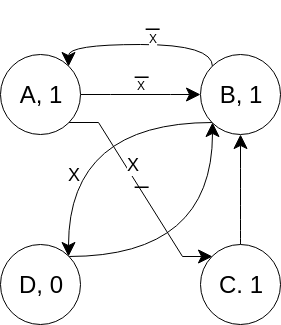
\includegraphics[width=0.3\textwidth]{diagram.png}	
	\caption{State diagram}
	\label{circ:part1b}
\end{figure}


% \begin{align}
% F_{4}(a,b,c,d) &= (a   b   c'   d) \notag\\ 
% &= (a b' c' d) + (abc'd) + (a'b'cd') + (a'bcd') + (a'   b'   c'   d) + (a'   b   c'   d) + (a   b'   c   d') + (a   b   c   d') \tag{Commutativity} \\
% &= ac'd(b' + b) + a'cd'(b'+b) + a'c'd(b' + b) + acd'(b'+b) \tag{Distribution} \\
% &= ac'd(1) + a'cd'(1) + a'c'd(1) + acd'(1) \tag{Inverse} \\
% &= ac'd + a'cd'+ a'c'd+ acd' \tag{Identitiy} \\
% &= ac'd + a'c'd + a'cd' + acd' \tag{Commutativity} \\
% &= c'd(a + a') + cd'(a' + a) \tag{Distribution} \\
% &= c'd + cd' \notag
% \end{align}







\end{flushleft}
\newpage
\begin{flushleft}
\subsection{PART 2}
\paragraph{}
In the next part of the experiment, a 2-bit counter circuit that counts from 0 to 2 in a circular way is designed and implemented as shown in the figure below.  When X input value is 1, the circuit is counting UP,  when X input value is 0, the circuit is counting down.  The clock is connected to a debounced push-button. 

\begin{figure}[h]
	\centering
	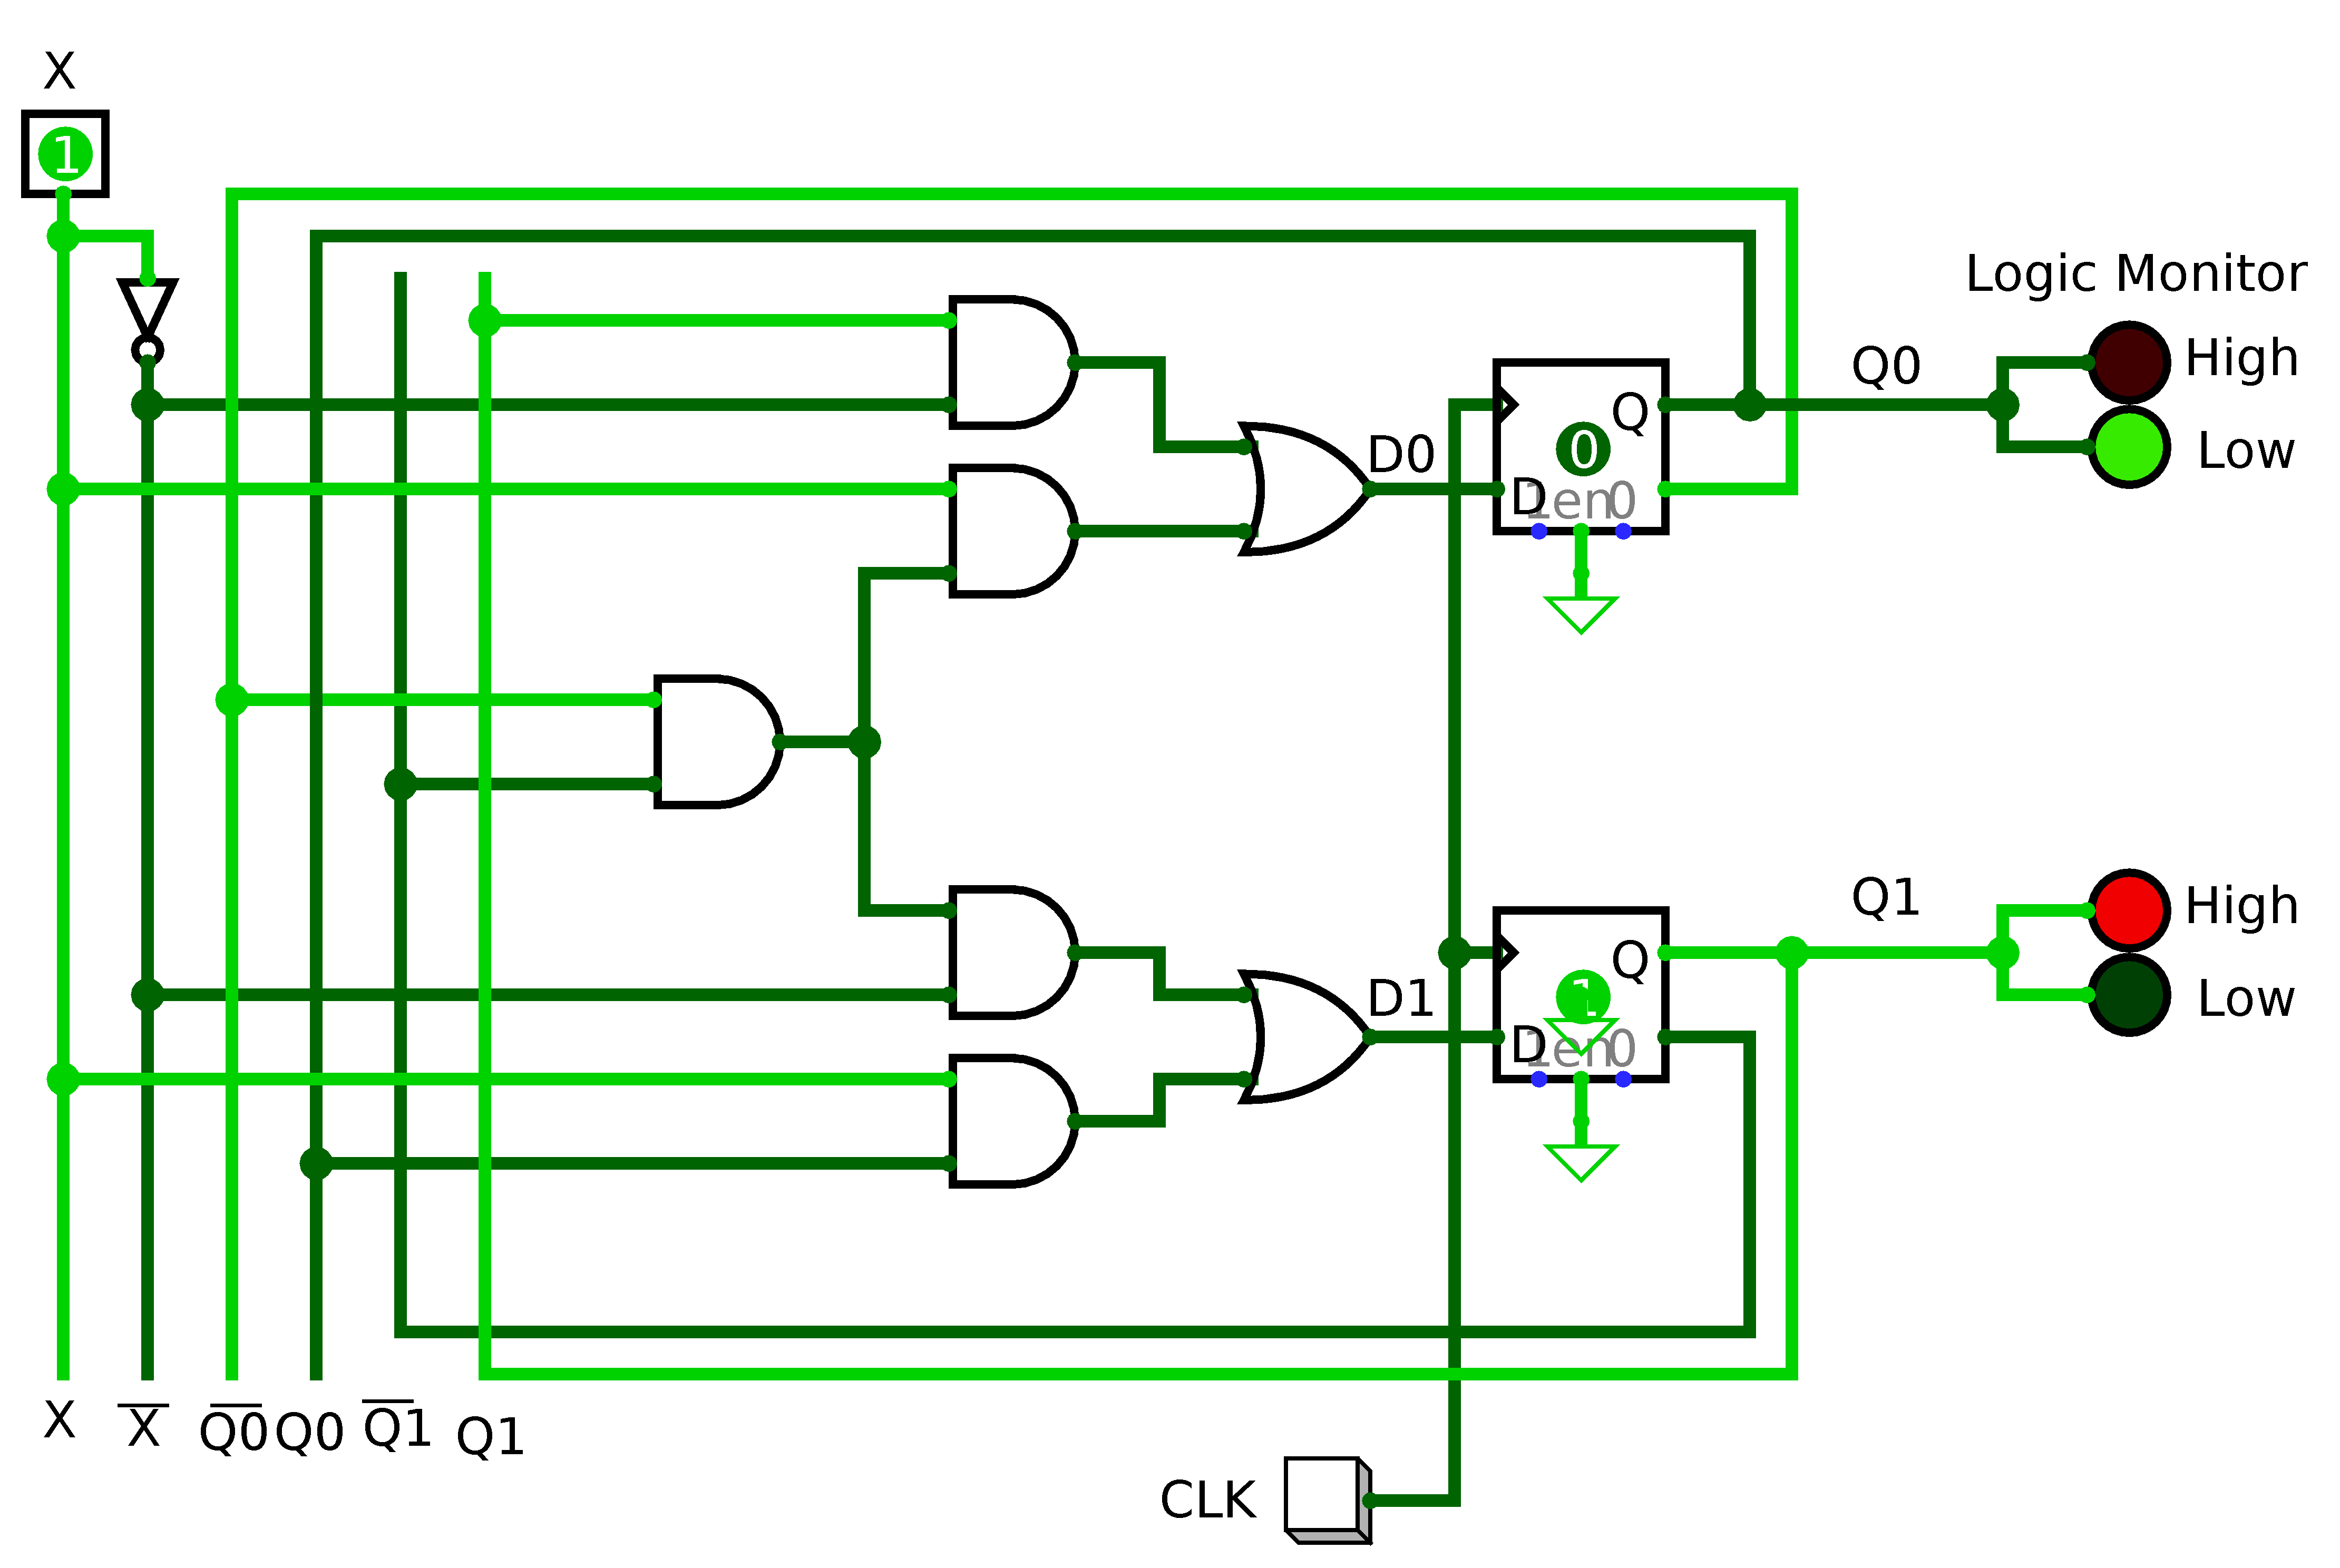
\includegraphics[width=0.7\textwidth]{part2.png}	
	\caption{Counter that can count up and down depending on X}
	\label{circ:part2}
\end{figure}

\newpage

% Please add the following required packages to your document preamble:
% \usepackage{multirow}
\begin{table}[h]
\centering
\begin{tabular}{cc|cc}
\multicolumn{2}{c|}{\multirow{2}{*}{$Q^{+}_{1}Q^{+}_{0}$}} & \multicolumn{2}{c}{X}   \\
\multicolumn{2}{c|}{}                                      & 0          & 1          \\ \hline
\multirow{4}{*}{$Q_{1}Q_{0}$}             & 00             & 10         & 01         \\
                                          & 01             & 00         & 10         \\
                                          & 10             & 01         & 00         \\
                                          & 11             & $\phi\phi$ & $\phi\phi$
\end{tabular}
\caption{State transition table}
\label{tab:part2}
\end{table}




% Please add the following required packages to your document preamble:
% \usepackage{multirow}
\begin{table}[h]
\centering
\begin{tabular}{cc|cc}
\multicolumn{2}{c|}{\multirow{2}{*}{$Q_{1}Q^{+}_{1}$}} & \multicolumn{2}{c}{X}   \\
\multicolumn{2}{c|}{}                                  & 0          & 1          \\ \hline
\multirow{4}{*}{$Q_{1}Q_{0}$}           & 00           & 01         & 00         \\
                                        & 01           & 00         & 01         \\
                                        & 10           & 10         & 10         \\
                                        & 11           & $\phi\phi$ & $\phi\phi$
\end{tabular}
\caption{Transition of table $Q_{1}$}
\label{tab:part2_q1}
\end{table}




% Please add the following required packages to your document preamble:
% \usepackage{multirow}

\begin{table}[h]
\centering
\begin{tabular}{cc|cc}
\multicolumn{2}{c|}{\multirow{2}{*}{$Q_{1}Q^{+}_{1}$}} & \multicolumn{2}{c}{X}   \\
\multicolumn{2}{c|}{}                                  & 0          & 1          \\ \hline
\multirow{4}{*}{$Q_{1}Q_{0}$}           & 00           & $\alpha$   & 0          \\
                                        & 01           & 0          & $\alpha$   \\
                                        & 10           & $\beta$    & $\beta$    \\
                                        & 11           & $\phi\phi$ & $\phi\phi$
\end{tabular}
\caption{Transition of table $Q_{1}$}
\label{tab:part2_q1_2}
\end{table}


%\end{flushleft}


\newpage

% Please add the following required packages to your document preamble:
% \usepackage{multirow}
\begin{table}[h]
\centering
\begin{tabular}{cc|cc}
\multicolumn{2}{c|}{\multirow{2}{*}{$Q_{0}Q^{+}_{0}$}} & \multicolumn{2}{c}{X}   \\
\multicolumn{2}{c|}{}                                  & 0          & 1          \\ \hline
\multirow{4}{*}{$Q_{1}Q_{0}$}           & 00           & 00         & 01         \\
                                        & 01           & 10         & 10         \\
                                        & 10           & 01         & 00         \\
                                        & 11           & $\phi\phi$ & $\phi\phi$
\end{tabular}
\caption{Transition of table $Q_{0}$}
\label{tab:part2_q0}
\end{table}

\end{flushleft}
% Please add the following required packages to your document preamble:
% \usepackage{multirow}
\begin{table}[h]
\centering
\begin{tabular}{cc|cc}
\multicolumn{2}{c|}{\multirow{2}{*}{$Q_{0}Q^{+}_{0}$}} & \multicolumn{2}{c}{X}   \\
\multicolumn{2}{c|}{}                                  & 0          & 1          \\ \hline
\multirow{4}{*}{$Q_{1}Q_{0}$}           & 00           & 0          & $\alpha$   \\
                                        & 01           & $\beta$    & $\beta$    \\
                                        & 10           & $\alpha$   & 0          \\
                                        & 11           & $\phi\phi$ & $\phi\phi$
\end{tabular}
\caption{Transition of table $Q_{0}$}
\label{tab:part2_q1}
\end{table}


\begin{table}[h]
\centering
\begin{tabular}{cc|c}
symbol   & $QQ^{+}$ & D \\ \hline
0        & 00       & 0 \\
$\alpha$ & 01       & 1 \\
$\beta$  & 10       & 0 \\
1        & 11       & 1
\end{tabular}
\caption{D flip-flop transition}ta
\ebllabel{tab:part 2_d}
\end{table}


\begin{table}[h]
\centering
\begin{tabular}{cc|cc}
\multicolumn{2}{c|}{\multirow{2}{*}{$D_{1}$}} & \multicolumn{2}{c}{X}   \\
\multicolumn{2}{c|}{}                         & 0          & 1          \\ \hline
\multirow{4}{*}{$Q_{1}Q_{0}$}       & 00      & 1          & 0          \\
                                    & 01      & 0          & 1          \\
                                    & 11      & $\phi\phi$ & $\phi\phi$ \\
                                    & 10      & 0          & 0         
\end{tabular}
\caption{Karnaugh diagram for $D_{1}$}
\label{tab:part2_d}
\end{table}

\begin{table}[h]
\centering
\begin{tabular}{cc|cc}
\multicolumn{2}{c|}{\multirow{2}{*}{$D_{0}$}} & \multicolumn{2}{c}{X}   \\
\multicolumn{2}{c|}{}                         & 0          & 1          \\ \hline
\multirow{4}{*}{$Q_{1}Q_{0}$}       & 00      & 0          & 1          \\
                                    & 01      & 0          & 0          \\
                                    & 11      & $\phi\phi$ & $\phi\phi$ \\
                                    & 10      & 1          & 0         
\end{tabular}
\caption{Karnaugh diagram for $D_{0}$}
\label{tab:part2_d}
\end{table}


Expressions of inputs of D flip flops:
\begin{align}
    D_{1} &= X \cdot Q_{0} + \bar{Q_{0}} \cdot \bar{Q_{1}} \cdot \bar{X} \notag \\
    D_{0} &= \bar{X} \cdot Q_{1} + \bar{Q_{0}} \cdot \bar{Q_{1}} \cdot X \notag \\
\end{align}


% D_{0}
% D_{1}
% \bar{D_{0}}
% \bar{D_{1}}

% Q_{0}
% Q_{1}
% \bar{Q_{0}}
% \bar{Q_{0}}

% Q^{+}_{0}
% Q^{+}_{1}






\begin{flushleft}
 
 
\subsection{PART 3}

\paragraph{}
In the final part of the experiment,  a counter that counts from 0 to 5 in a circular way is implemented using the 74xx161 IC. Output values are observed using the seven segment display

 \newpage
\begin{figure}[h]
	\centering
	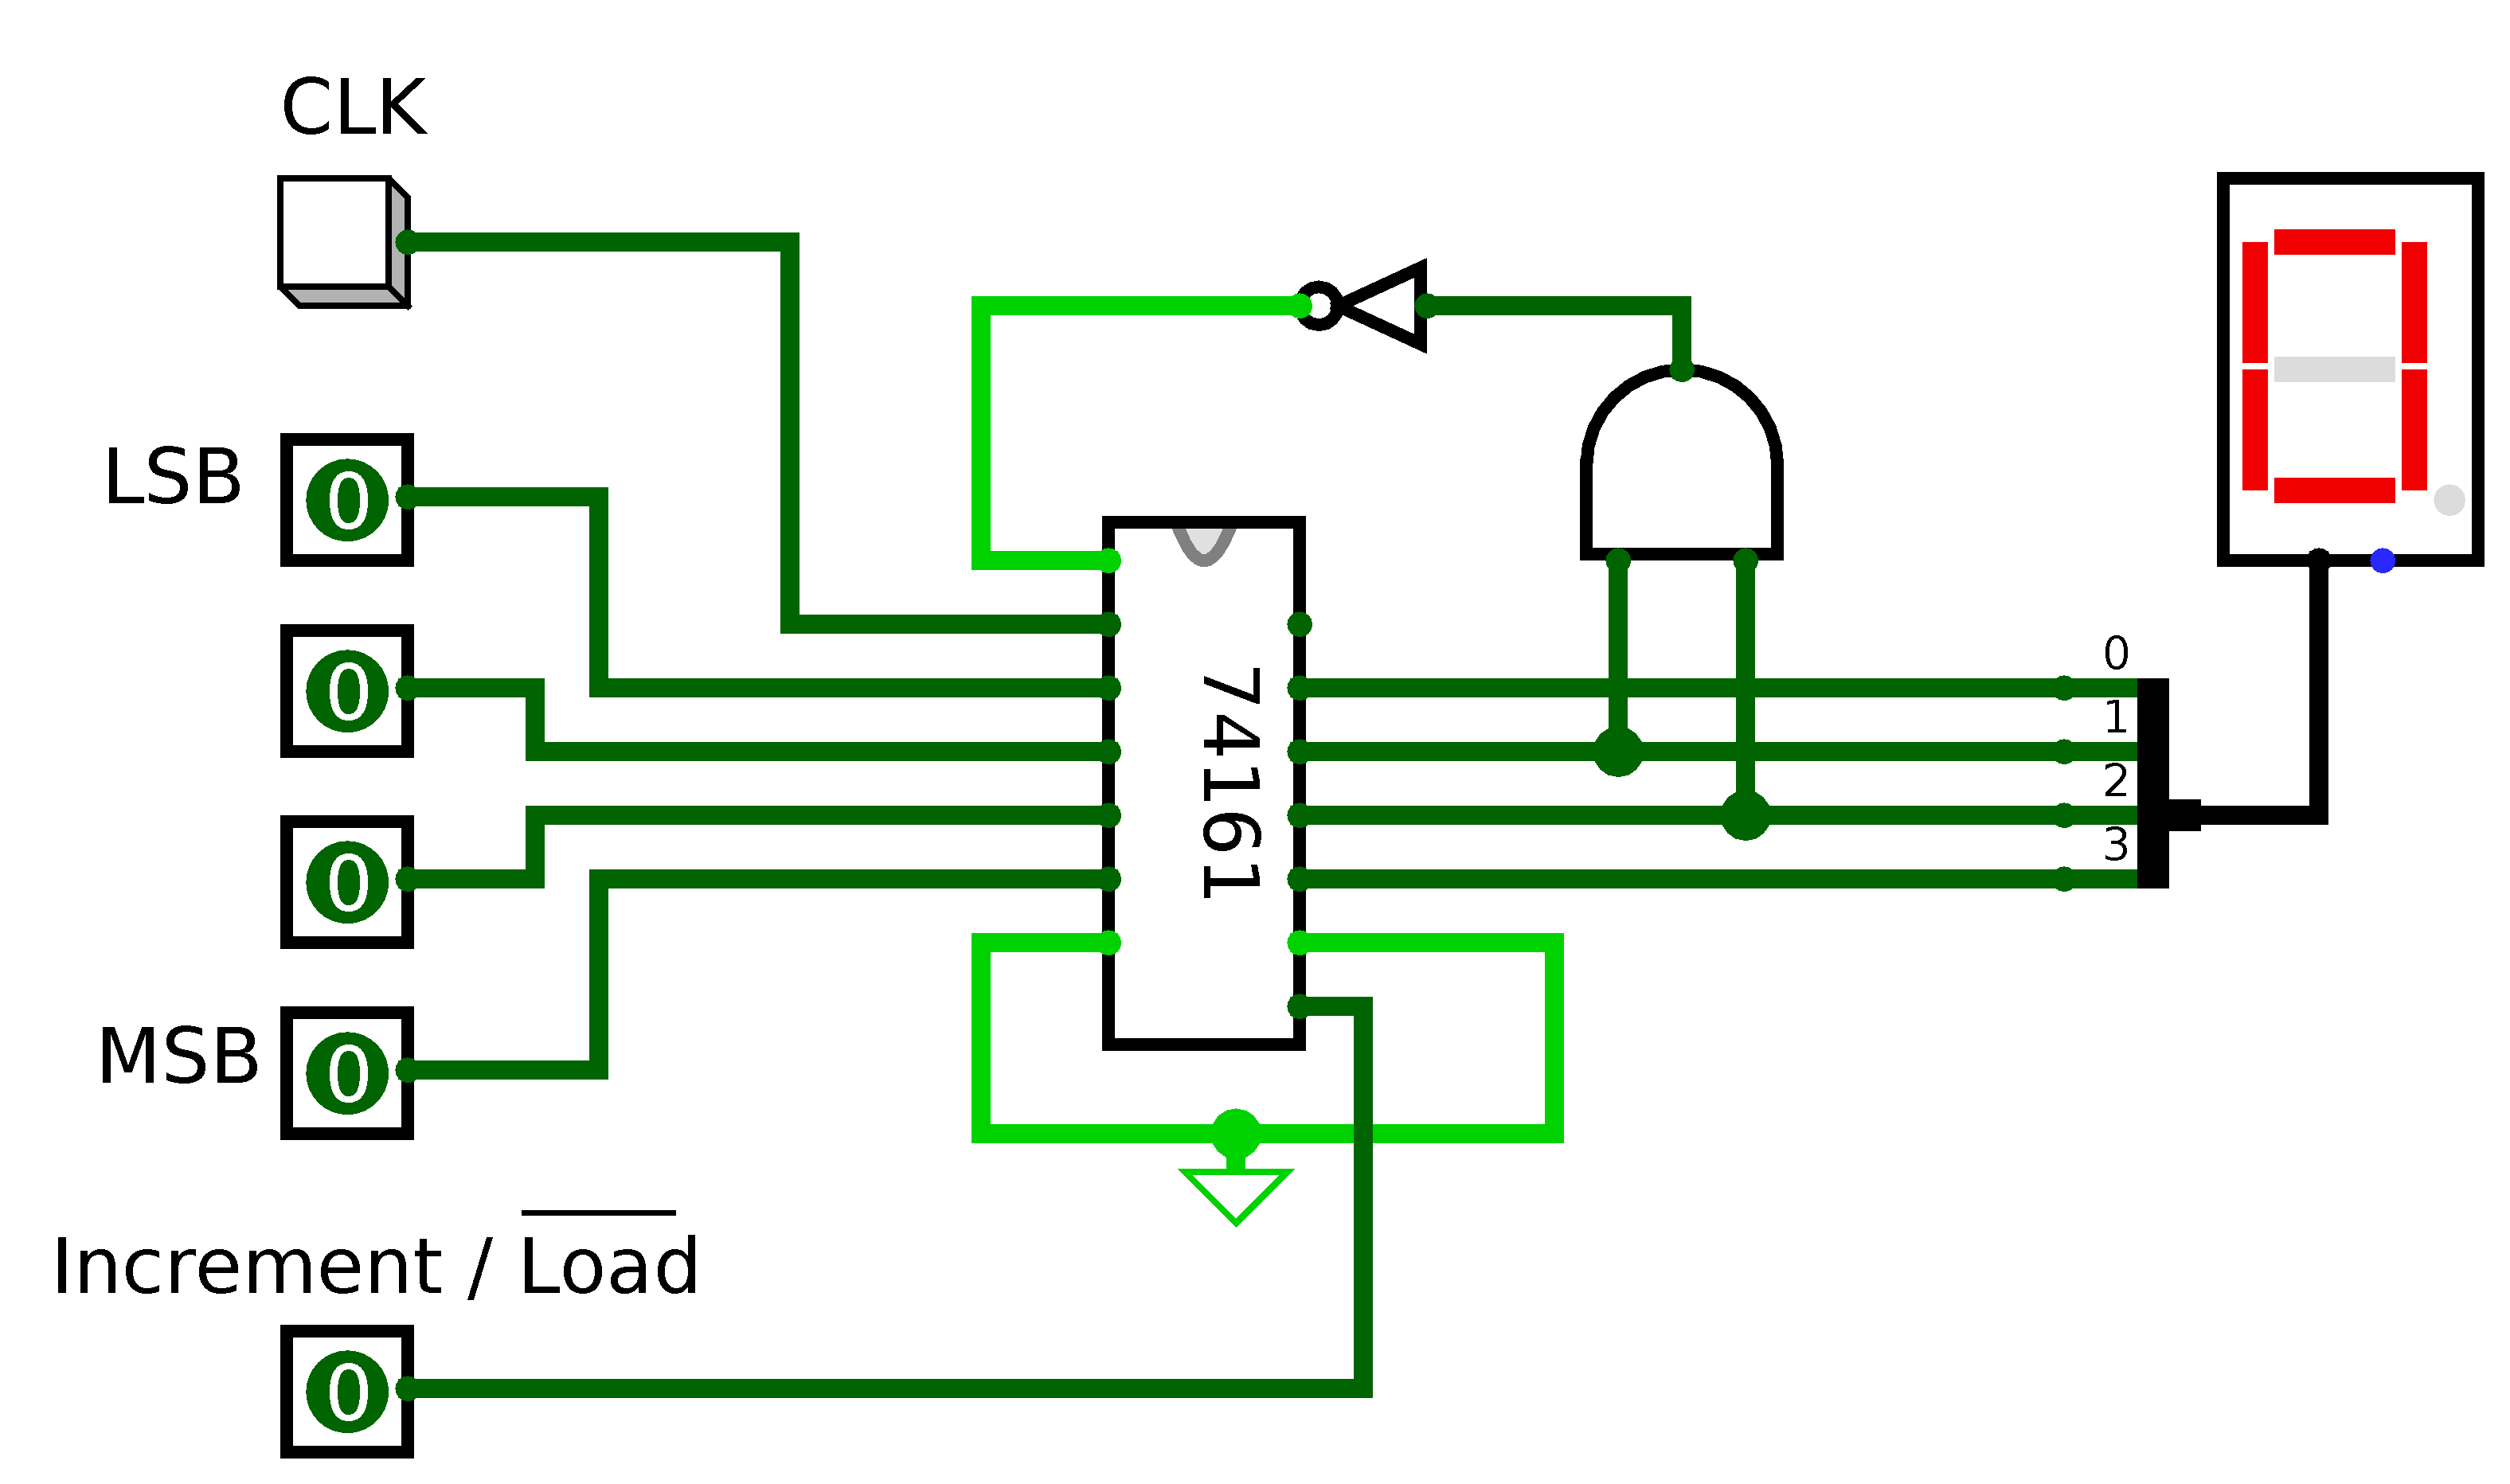
\includegraphics[width=0.7\textwidth]{part3.png}	
	\caption{Circuit for counting from 0 to 5}
	\label{circ:part3}
\end{figure}
\end{flushleft}











\section{INTERPRETATION OF THE RESULTS}
\begin{flushleft}



\paragraph {}
For the first part of the experiment, we did implement the circuit without facing any issues. The results we observed were consistent with the truth tables we have constructed beforehand. While implementing part 2 however, we ran into an issue that we couldn't find the resolution to. Our counter could count up but would go from 2 to 0 when counting down and then wouldn't cycle. While doing part 3 of the experiment, we have encountered another rather interesting occurrence. We implemented the counter that was described in the experiment booklet. It did work when the clock signal was frequent but didn't when it had a really low frequency. A few other lab groups also were having the same issue. We weren't able to determine its reason for sure but we believe it might be caused by different propagation delays of the units used.

%oh shit zaman bitiyo abi cidden planımız ne??

% yaz abi bisiler xd ben o kismi yapiyorum ztn tablolari filan hepsini koyuyorum onlari hallettim part1 e bi bak part2 yi de hallediyorum simdi
\end{flushleft}

\section{CONCLUSION}

\begin{flushleft}

% Buralardan emin degilim cihat yazmis onceki deneye gore
 \paragraph {}
 We were not able to finish part 2 of the experiment which we addressed in detail in previous parts. Even though we had an issue with that part, this experiment helped us understand the working mechanism of a counter better. 
 \newline We also believe that, being more efficient with time will allow us to be more successful in future experiment.
\end{flushleft}


\nocite{overleaf}
\nocite{reportGuide}

 

\newpage
\addcontentsline{toc}{section}{\numberline {}REFERENCES}

\bibliographystyle{unsrt}
\bibliography{reference}

\end{document}

